\begin{IEEEbiography}{Ganesh Venkatraman}
	(S'14) received the B.E. degree in electronics and communications engineering from the Madras University, Chennai, India in 2003, and the M.S. degree in electrical engineering from the Indian Institute of Technology (IIT) Madras, Chennai, India in 2006. He is currently pursuing the Dr. Sc. (Tech.) degree in the Department of Communication Engineering (DCE), Centre for Wireless Communications (CWC), University of Oulu, Oulu, Finland. %Prior to this, he worked as a Design Engineer in the Freescale Semiconductor India Pvt. Ltd., Noida, India during the year (2010-2011) and as a Research Engineer at the Center of Excellence in Wireless Technology (CEWiT), Chennai, India during the year (2008-2010). 
	His research interests include radio resource management, transceiver algorithms for wireless communications, and signal processing techniques in baseband implementation.
\end{IEEEbiography}

\begin{IEEEbiography}[{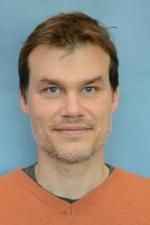
\includegraphics[trim=0cm 1.2cm 0.2cm 0.3cm,clip,scale=0.52]{TolliAntti_0.jpg}}]{Antti T\"olli}
(M'08, SM'14) received the Dr.Sc. (Tech.) degree in electrical engineering from the University of Oulu, Oulu, Finland, in 2008. Before joining the Department of Communication Engineering (DCE) and Centre for Wireless Communications (CWC) at the University of Oulu, he worked for 5 years with Nokia Networks, IP Mobility Networks Division, as a Research Engineer and Project Manager both in Finland and Spain. In May 2014, he was granted a five year (2014--2019) Academy Research Fellow post by the Research Council for Natural Sciences and Engineering of the Academy of Finland. He also holds an Adjunct Professor position with the DCE, University of Oulu. During the academic year 2015-2016, he holds a visiting position at EURECOM, Sophia Antipolis, France. He has authored more than 120 papers in peer-reviewed international journals and conferences and several patents all in the area
of signal processing and wireless communications. His research interests include radio resource management and transceiver design for broadband wireless communications with a special emphasis on distributed interference management in heterogeneous wireless networks. 
\end{IEEEbiography}

\begin{IEEEbiography}[{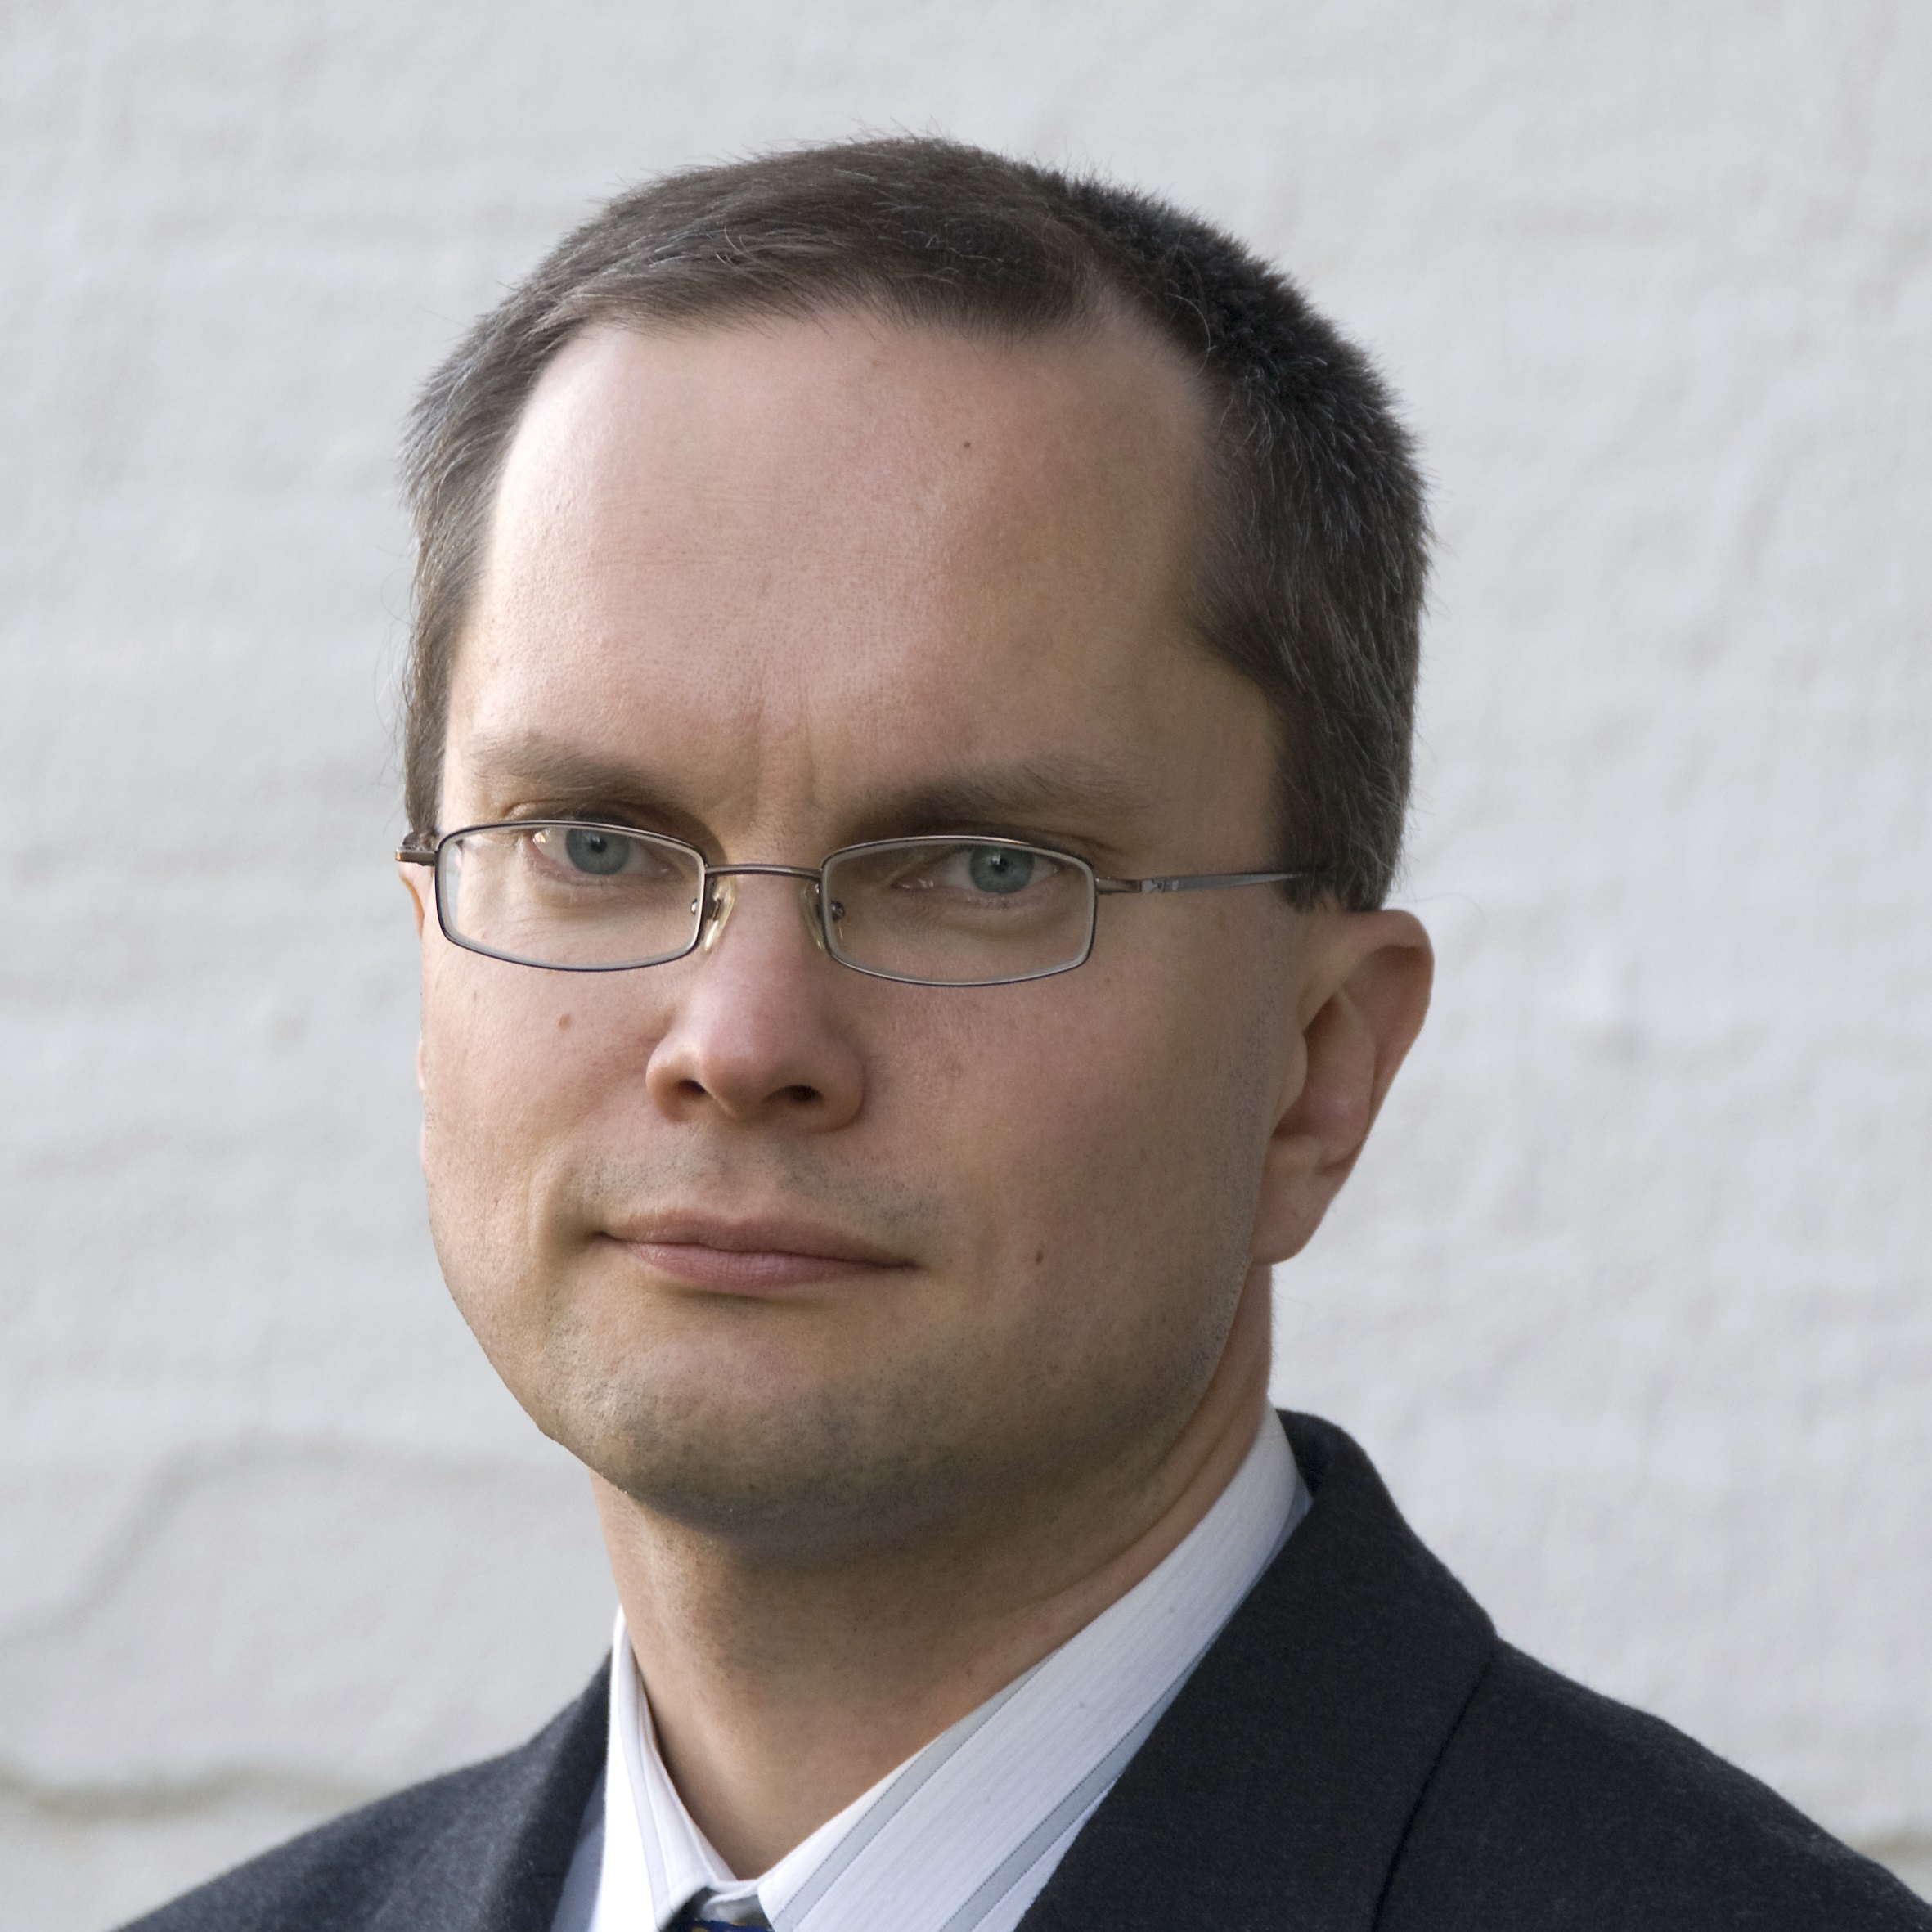
\includegraphics[trim=2cm 1cm 3cm 1cm,clip,scale=0.18]{Markku_Juntti_200x200mm.jpg}}]{Markku Juntti}
(S'93-M'98-SM'04) received his M.Sc.\ (EE) and Dr.Sc.\ (EE) degrees from University of Oulu, Oulu, Finland in 1993 and 1997, respectively.
	
Dr.\ Juntti was with University of Oulu in 1992--98. In academic year 1994--95, he was a Visiting Scholar at Rice University, Houston, Texas. In 1999--2000, he was a Senior Specialist with Nokia Networks. Dr.\ Juntti has been a a professor of communications engineering since 2000 at University of Oulu, Department of Communication Engineering (DCE) and Centre for Wireless Communications (CWC), where he leads the Communications Signal Processing (CSP) Research Group. In 2014--2017, he also serves as Dean of University of Oulu Graduate School. His research interests include signal processing for wireless networks as well as communication and information theory. He is an author or co-author in some 350 papers published in international journals and conference records as well as in books {\it WCDMA for UMTS} and {\it Signal Processing Handbook}. Dr.\ Juntti is also an Adjunct Professor at Department of Electrical and Computer Engineering, Rice University, Houston, Texas, USA.
	
Dr.\ Juntti is an Editor of \textsc{IEEE Transactions on Communications} and was an Associate Editor for \textsc{IEEE Transactions on Vehicular Technology} in 2002--2008. He was Secretary of IEEE Communication Society Finland Chapter in 1996--97 and the Chairman for years 2000--01. He has been Secretary of the Technical Program Committee (TPC) of the 2001 IEEE International Conference on Communications (ICC'01), and the Co-Chair of the Technical Program Committee of 2004 Nordic Radio Symposium and 2006 IEEE International Symposium on Personal, Indoor and Mobile Radio Communications (PIMRC 2006), and the General Chair of 2011 IEEE Communication Theory Workshop (CTW 2011). He has served as Co-Chair of the Signal Processing for Communications Symposium of GLOBECOM 2014.
\end{IEEEbiography}

\begin{IEEEbiography}[{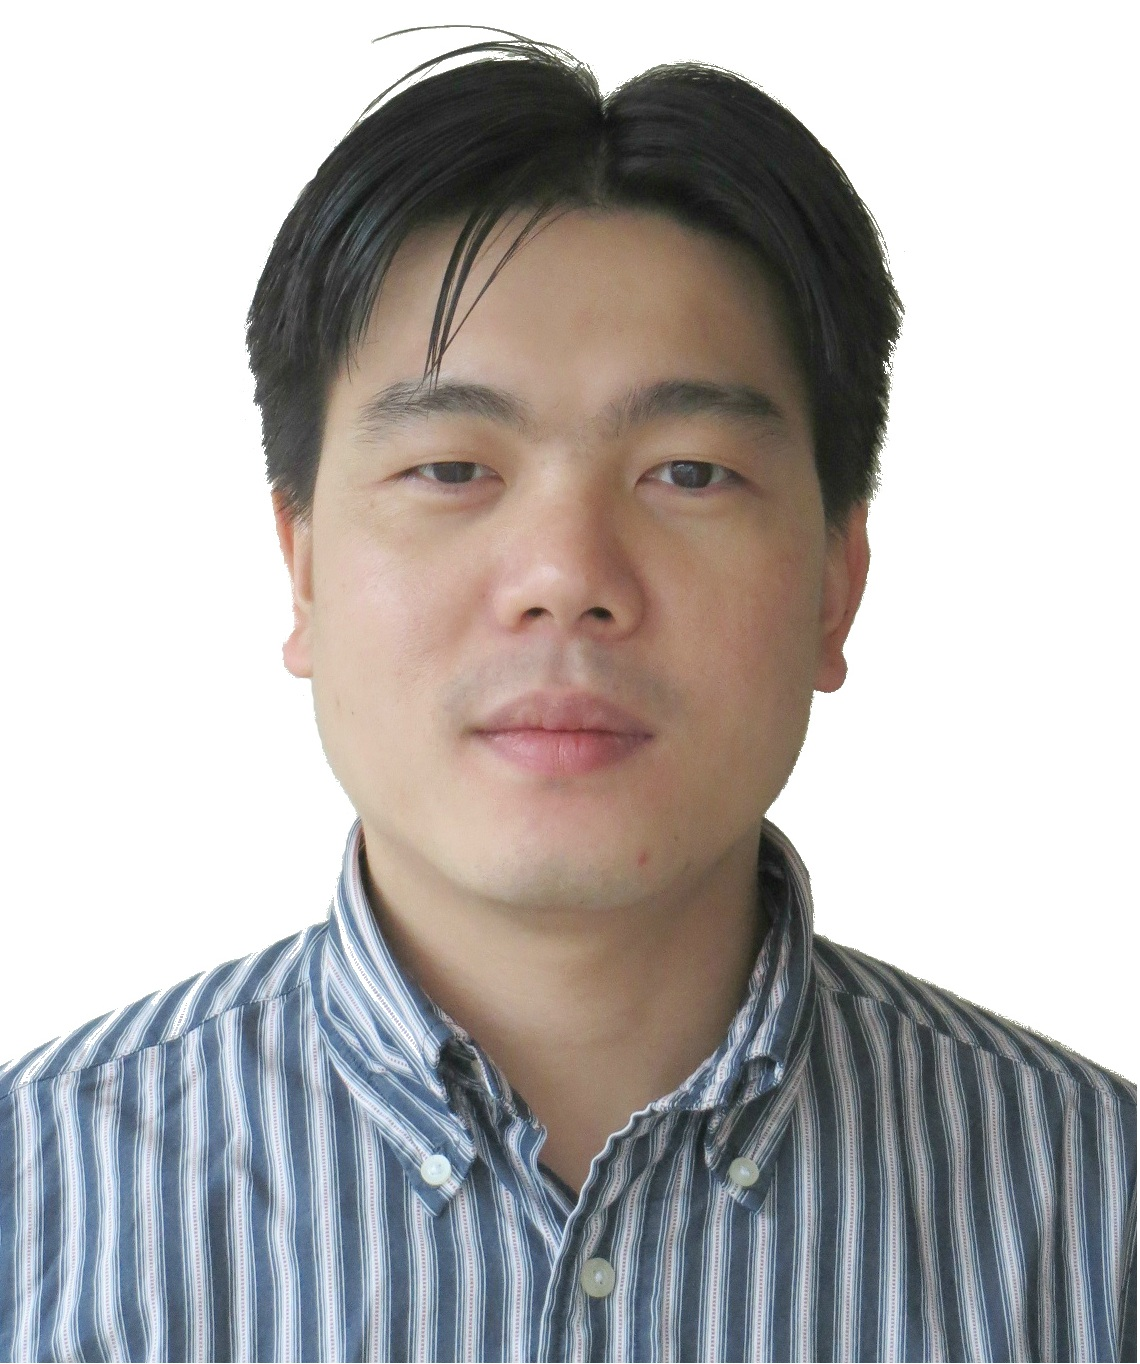
\includegraphics[trim=0cm 0cm 0.5cm 0cm,clip,scale=0.094]{Nam_Tran.jpg}}]{Le-Nam Tran}
	(M'10) received the B.S. degree in electrical engineering from Ho Chi Minh City University of Technology, Ho Chi Minh City, Vietnam, in 2003 and the M.S. and Ph.D. degrees in radio engineering from Kyung Hee University, Seoul, Korea, in 2006 and 2009, respectively. In 2009, he joined the Department of Electrical Engineering, Kyung Hee University, as a Lecturer. From 2010 to 2014, he had held postdoctoral positions at the Signal Processing Laboratory, ACCESS Linnaeus Centre, KTH Royal Institute of Technology, Sweden and the Centre for Wireless Communications and the Department of Communications Engineering, University of Oulu, Finland. Since Sep. 2014, he has been a lecturer at the Department of Electronic Engineering, Maynooth University, Co. Kildare, Ireland. His current research interests include multiuser MIMO systems, energy-efficient communications, full-duplex transmission, and applications of optimization techniques.
\end{IEEEbiography}
